% Options for packages loaded elsewhere
\PassOptionsToPackage{unicode}{hyperref}
\PassOptionsToPackage{hyphens}{url}
\PassOptionsToPackage{dvipsnames,svgnames,x11names}{xcolor}
%
\documentclass[
  letterpaper,
  DIV=11,
  numbers=noendperiod]{scrartcl}

\usepackage{amsmath,amssymb}
\usepackage{iftex}
\ifPDFTeX
  \usepackage[T1]{fontenc}
  \usepackage[utf8]{inputenc}
  \usepackage{textcomp} % provide euro and other symbols
\else % if luatex or xetex
  \usepackage{unicode-math}
  \defaultfontfeatures{Scale=MatchLowercase}
  \defaultfontfeatures[\rmfamily]{Ligatures=TeX,Scale=1}
\fi
\usepackage{lmodern}
\ifPDFTeX\else  
    % xetex/luatex font selection
\fi
% Use upquote if available, for straight quotes in verbatim environments
\IfFileExists{upquote.sty}{\usepackage{upquote}}{}
\IfFileExists{microtype.sty}{% use microtype if available
  \usepackage[]{microtype}
  \UseMicrotypeSet[protrusion]{basicmath} % disable protrusion for tt fonts
}{}
\makeatletter
\@ifundefined{KOMAClassName}{% if non-KOMA class
  \IfFileExists{parskip.sty}{%
    \usepackage{parskip}
  }{% else
    \setlength{\parindent}{0pt}
    \setlength{\parskip}{6pt plus 2pt minus 1pt}}
}{% if KOMA class
  \KOMAoptions{parskip=half}}
\makeatother
\usepackage{xcolor}
\setlength{\emergencystretch}{3em} % prevent overfull lines
\setcounter{secnumdepth}{-\maxdimen} % remove section numbering
% Make \paragraph and \subparagraph free-standing
\makeatletter
\ifx\paragraph\undefined\else
  \let\oldparagraph\paragraph
  \renewcommand{\paragraph}{
    \@ifstar
      \xxxParagraphStar
      \xxxParagraphNoStar
  }
  \newcommand{\xxxParagraphStar}[1]{\oldparagraph*{#1}\mbox{}}
  \newcommand{\xxxParagraphNoStar}[1]{\oldparagraph{#1}\mbox{}}
\fi
\ifx\subparagraph\undefined\else
  \let\oldsubparagraph\subparagraph
  \renewcommand{\subparagraph}{
    \@ifstar
      \xxxSubParagraphStar
      \xxxSubParagraphNoStar
  }
  \newcommand{\xxxSubParagraphStar}[1]{\oldsubparagraph*{#1}\mbox{}}
  \newcommand{\xxxSubParagraphNoStar}[1]{\oldsubparagraph{#1}\mbox{}}
\fi
\makeatother


\providecommand{\tightlist}{%
  \setlength{\itemsep}{0pt}\setlength{\parskip}{0pt}}\usepackage{longtable,booktabs,array}
\usepackage{calc} % for calculating minipage widths
% Correct order of tables after \paragraph or \subparagraph
\usepackage{etoolbox}
\makeatletter
\patchcmd\longtable{\par}{\if@noskipsec\mbox{}\fi\par}{}{}
\makeatother
% Allow footnotes in longtable head/foot
\IfFileExists{footnotehyper.sty}{\usepackage{footnotehyper}}{\usepackage{footnote}}
\makesavenoteenv{longtable}
\usepackage{graphicx}
\makeatletter
\def\maxwidth{\ifdim\Gin@nat@width>\linewidth\linewidth\else\Gin@nat@width\fi}
\def\maxheight{\ifdim\Gin@nat@height>\textheight\textheight\else\Gin@nat@height\fi}
\makeatother
% Scale images if necessary, so that they will not overflow the page
% margins by default, and it is still possible to overwrite the defaults
% using explicit options in \includegraphics[width, height, ...]{}
\setkeys{Gin}{width=\maxwidth,height=\maxheight,keepaspectratio}
% Set default figure placement to htbp
\makeatletter
\def\fps@figure{htbp}
\makeatother
% definitions for citeproc citations
\NewDocumentCommand\citeproctext{}{}
\NewDocumentCommand\citeproc{mm}{%
  \begingroup\def\citeproctext{#2}\cite{#1}\endgroup}
\makeatletter
 % allow citations to break across lines
 \let\@cite@ofmt\@firstofone
 % avoid brackets around text for \cite:
 \def\@biblabel#1{}
 \def\@cite#1#2{{#1\if@tempswa , #2\fi}}
\makeatother
\newlength{\cslhangindent}
\setlength{\cslhangindent}{1.5em}
\newlength{\csllabelwidth}
\setlength{\csllabelwidth}{3em}
\newenvironment{CSLReferences}[2] % #1 hanging-indent, #2 entry-spacing
 {\begin{list}{}{%
  \setlength{\itemindent}{0pt}
  \setlength{\leftmargin}{0pt}
  \setlength{\parsep}{0pt}
  % turn on hanging indent if param 1 is 1
  \ifodd #1
   \setlength{\leftmargin}{\cslhangindent}
   \setlength{\itemindent}{-1\cslhangindent}
  \fi
  % set entry spacing
  \setlength{\itemsep}{#2\baselineskip}}}
 {\end{list}}
\usepackage{calc}
\newcommand{\CSLBlock}[1]{\hfill\break\parbox[t]{\linewidth}{\strut\ignorespaces#1\strut}}
\newcommand{\CSLLeftMargin}[1]{\parbox[t]{\csllabelwidth}{\strut#1\strut}}
\newcommand{\CSLRightInline}[1]{\parbox[t]{\linewidth - \csllabelwidth}{\strut#1\strut}}
\newcommand{\CSLIndent}[1]{\hspace{\cslhangindent}#1}

\KOMAoption{captions}{tableheading}
\makeatletter
\@ifpackageloaded{caption}{}{\usepackage{caption}}
\AtBeginDocument{%
\ifdefined\contentsname
  \renewcommand*\contentsname{Table of contents}
\else
  \newcommand\contentsname{Table of contents}
\fi
\ifdefined\listfigurename
  \renewcommand*\listfigurename{List of Figures}
\else
  \newcommand\listfigurename{List of Figures}
\fi
\ifdefined\listtablename
  \renewcommand*\listtablename{List of Tables}
\else
  \newcommand\listtablename{List of Tables}
\fi
\ifdefined\figurename
  \renewcommand*\figurename{Figure}
\else
  \newcommand\figurename{Figure}
\fi
\ifdefined\tablename
  \renewcommand*\tablename{Table}
\else
  \newcommand\tablename{Table}
\fi
}
\@ifpackageloaded{float}{}{\usepackage{float}}
\floatstyle{ruled}
\@ifundefined{c@chapter}{\newfloat{codelisting}{h}{lop}}{\newfloat{codelisting}{h}{lop}[chapter]}
\floatname{codelisting}{Listing}
\newcommand*\listoflistings{\listof{codelisting}{List of Listings}}
\makeatother
\makeatletter
\makeatother
\makeatletter
\@ifpackageloaded{caption}{}{\usepackage{caption}}
\@ifpackageloaded{subcaption}{}{\usepackage{subcaption}}
\makeatother

\ifLuaTeX
  \usepackage{selnolig}  % disable illegal ligatures
\fi
\usepackage{bookmark}

\IfFileExists{xurl.sty}{\usepackage{xurl}}{} % add URL line breaks if available
\urlstyle{same} % disable monospaced font for URLs
\hypersetup{
  pdftitle={Predicing Level of Acceptability of Cars using Machine Learning},
  pdfauthor={Danish Karlin Isa \& Nicholas Varabioff \& Ximin Xu \& Zuer Zhong},
  colorlinks=true,
  linkcolor={blue},
  filecolor={Maroon},
  citecolor={Blue},
  urlcolor={Blue},
  pdfcreator={LaTeX via pandoc}}


\title{Predicing Level of Acceptability of Cars using Machine Learning}
\author{Danish Karlin Isa \& Nicholas Varabioff \& Ximin Xu \& Zuer
Zhong}
\date{2024-12-06}

\begin{document}
\maketitle

\renewcommand*\contentsname{Table of contents}
{
\hypersetup{linkcolor=}
\setcounter{tocdepth}{2}
\tableofcontents
}

by Danish Karlin Isa, Nicholas Varabioff, Ximin Xu, Zuer Zhong

\subsection{Summary}\label{summary}

In this project, we attempt to predict the level of acceptability of
cars by building a machine learning model. To choose the best model for
this task, we utilised several common machine learning models, and found
out that the SVM RBF classifier achieved the best train and
cross-validation scores, with a test accuracy of 0.952. On the 346 test
data cases, it correctly predicted the targets of 343 examples, while
there were only 3 examples with incorrect predicted targets.

The SVM RBF model also showed exceptional ability in determining the
acceptability of cars as seen in the confusion matrix, classification
reports, and relatively high scores for precision, recall and F1.
However, a slight decrease in classification precision was observed for
the ``good'' category, together with a relatively lower recall score of
0.86 that indicates occasional classification errors. Nonetheless, the
results obtained from this analysis further exemplifies the ability of
the SVM RBF model in handling nonlinear decision boundaries. This makes
the SVM RBF model a solid choice for this project.

\subsection{Introduction}\label{introduction}

The Car Evaluation Dataset was created as part of efforts to understand
the factors that affect the acceptability of cars among consumers. These
factors include buying price of a car, maintenance costs, passenger and
luggage capacity, and safety. The goal of this project is to develop a
machine learning model that can evaluate the quality of a car based on
its attributes to help buyers make a more informed decision for their
next car purchase.

The RBF SVM model is known for its effectiveness in nonlinear
classification tasks, and its use is particularly useful at navigating
the complexities of car evaluation. We expected the model to perform
well. In our tests, we also found that it outperformed other models such
as Naive Bayes and logistic regression. Our findings suggest a potential
class imbalance or capacity limitation in the model's ability to
adequately capture the nuances of the ``good'' classes. This raises
questions about the ideal modeling approach for such datasets.

\subsection{Methods}\label{methods}

\subsubsection{Data}\label{data}

The dataset that was used in this project is of Car Evaluation Database
created by the efforts of M. Bohanec and V. Rajkovic in the early 1990s.
It is sourced from the UCI Machine Learning Repository and is publicly
available for research and can be found in the
\href{https://archive.ics.uci.edu/dataset/19/car+evaluation}{UCI Machine
Learning Repository}. Each row in the dataset details a car's attributes
(each feature is of categorical data type with several levels), which
includes:

\begin{itemize}
\tightlist
\item
  Buying price: \texttt{low}, \texttt{med}, \texttt{high},
  \texttt{vhigh}
\item
  Maintenance cost: \texttt{low}, \texttt{med}, \texttt{high},
  \texttt{vhigh}
\item
  Number of doors: \texttt{2}, \texttt{3}, \texttt{4}, \texttt{5more}
\item
  Seating capacity: \texttt{2}, \texttt{4}, \texttt{more}
\item
  Boot size: \texttt{small}, \texttt{med}, \texttt{big}
\item
  Safety rating: \texttt{low}, \texttt{med}, \texttt{high}
\end{itemize}

\subsubsection{Analysis}\label{analysis}

With the best model identified, the next step was to improve its
performance through hyperparameter optimization. Using
RandomizedSearchCV, a range of values for the SVM's hyperparameters C
and gamma were explored. This approach allowed for an efficient and
thorough search across the parameter space, and results in an optimal
esitimator to use.

The visualizations below, including a heatmap
((\textbf{heatmap\_tuning?})) of test scores obtained during
hyperparameter optimization. This interpretability aids in understanding
which parameters are most critical and how sensitive the model is to
these settings.

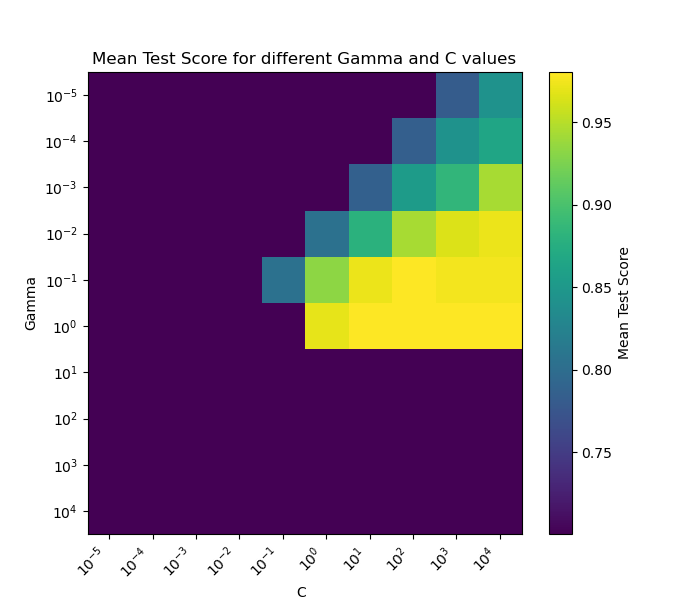
\includegraphics{../results/figures/car_hyperparameter.png}\{\#heatmap\_tuning,
width=100\%\}

We observed that the best hyperparameter of \(C\) and \(gamma\) are
100.0 and 0.1. All categorical features are one hot encoded prior to
model fitting. The Python programming language (Van Rossum and Drake
2009) and the following Python packages were used to perform the
analysis: numpy (Harris et al. 2020), Pandas (McKinney 2010), matplotlib
(Hunter 2007), scikit-learn (Pedregosa et al. 2011). The code used to
perform the analysis and create this report can be found here:
https://github.com/UBC-MDS/Car\_Evaluation\_Analysis/blob/main/scripts

\subsection{Results \& Discussion}\label{results-discussion}

After performing hyperparameter optimisation, the RBF SVM model with
\texttt{C=100.0} and \texttt{gamma=0.1} achieved the best performance on
the test set with a score of 0.99. This suggests the model has been
generalised well, with high scores on both the train and test sets.

To further improve the model's utility, several changes can be made. One
such change is feeding the model with features that are not just
categorical. Instead, for features such as buying price, maintenance
cost and safety features, numeric data should be used. At the same time,
more features can be included, such as the type of car and and fuel
efficiency ratings.

By allowing the model to take in more complex data, this may allow the
model to make more accurate predictions to let customers make a more
informed choice when purchasing a new car.

\begin{longtable}[]{@{}llllllll@{}}
\toprule\noalign{}
& buying & maint & doors & persons & lug\_boot & safety & class \\
\midrule\noalign{}
\endhead
\bottomrule\noalign{}
\endlastfoot
0 & vhigh & vhigh & 2 & 2 & small & low & unacc \\
1 & vhigh & vhigh & 2 & 2 & small & med & unacc \\
2 & vhigh & vhigh & 2 & 2 & small & high & unacc \\
3 & vhigh & vhigh & 2 & 2 & med & low & unacc \\
4 & vhigh & vhigh & 2 & 2 & med & med & unacc \\
\end{longtable}

\subsubsection{Data Import and
Validation}\label{data-import-and-validation}

\begin{longtable}[]{@{}llllllll@{}}
\toprule\noalign{}
& buying & maint & doors & persons & lug\_boot & safety & class \\
\midrule\noalign{}
\endhead
\bottomrule\noalign{}
\endlastfoot
0 & vhigh & vhigh & 2 & 2 & small & low & unacc \\
1 & vhigh & vhigh & 2 & 2 & small & med & unacc \\
2 & vhigh & vhigh & 2 & 2 & small & high & unacc \\
3 & vhigh & vhigh & 2 & 2 & med & low & unacc \\
4 & vhigh & vhigh & 2 & 2 & med & med & unacc \\
... & ... & ... & ... & ... & ... & ... & ... \\
1723 & low & low & 5more & more & med & med & good \\
1724 & low & low & 5more & more & med & high & vgood \\
1725 & low & low & 5more & more & big & low & unacc \\
1726 & low & low & 5more & more & big & med & good \\
1727 & low & low & 5more & more & big & high & vgood \\
\end{longtable}

Data validation checklist:

\begin{longtable}[]{@{}
  >{\raggedright\arraybackslash}p{(\columnwidth - 2\tabcolsep) * \real{0.4545}}
  >{\raggedright\arraybackslash}p{(\columnwidth - 2\tabcolsep) * \real{0.5455}}@{}}
\toprule\noalign{}
\begin{minipage}[b]{\linewidth}\raggedright
Check
\end{minipage} & \begin{minipage}[b]{\linewidth}\raggedright
Result
\end{minipage} \\
\midrule\noalign{}
\endhead
\bottomrule\noalign{}
\endlastfoot
Correct data file format & \texttt{car.data} does not have the right
extension, but can be read in as a \texttt{.csv} file \\
Correct column names & \texttt{car.data} does not contain column names;
column names located in \texttt{car.c45-names} and passed into
\texttt{columns=} argument in \texttt{pd.read\_csv()} \\
No empty observations & Passed \texttt{.validate} checks \\
Missingness not beyond expected threshold & Not applicable; no empty
observations (see above) \\
Correct data types in each column & Passed \texttt{.validate} checks \\
No duplicate observations & Passed \texttt{.validate} checks \\
No outlier or anomalous values & Not applicable; all features are
categorical \\
Correct category levels (i.e., no string mismatches or single values) &
Passed \texttt{.validate} checks \\
Target/response variable follows expected distribution & See Exploratory
Data Analysis \\
No anomalous correlations between target/response variable and
features/explanatory variables & See Preprocessing of Dataset \\
No anomalous correlations between features/explanatory variables & See
Preprocessing of Dataset \\
\end{longtable}

\subsubsection{Exploratory Data
Analysis}\label{exploratory-data-analysis}

Exploratory data analysis was carried out on the train dataset. Here,
the counts of records by target and category was visualised to gain a
better idea of the dataset.

\begin{verbatim}
<class 'pandas.core.frame.DataFrame'>
RangeIndex: 1728 entries, 0 to 1727
Data columns (total 7 columns):
 #   Column    Non-Null Count  Dtype 
---  ------    --------------  ----- 
 0   buying    1728 non-null   object
 1   maint     1728 non-null   object
 2   doors     1728 non-null   object
 3   persons   1728 non-null   object
 4   lug_boot  1728 non-null   object
 5   safety    1728 non-null   object
 6   class     1728 non-null   object
dtypes: object(7)
memory usage: 94.6+ KB
\end{verbatim}

\begin{verbatim}
alt.RepeatChart(...)
\end{verbatim}

Figure 1: Visualization of counts by feature and target class. Through
this analysis, we can see that examples with target class
\texttt{unacceptable} represent a large proportion of the dataset.

\subsection{Preprocessing of Dataset for Machine
Learning}\label{preprocessing-of-dataset-for-machine-learning}

We preprocess the dataset to prepare it for machine learning: Transform
categorical features using\texttt{OrdinalEncoder} . Split the dataset
into training and testing sets.

\begin{verbatim}
VBox(children=(HTML(value='<h4><b>Class Imbalance</b></h4>'), HTML(value='<p>Check if a dataset is imbalanced …
\end{verbatim}

\subsubsection{Model Selection}\label{model-selection}

The core of this project is choosing the appropriate machine learning
model. Thus, in the next step, several machine learning models will be
evaluated.

\texttt{cross\_validate} from \texttt{sklearn} will be used to evaluate
the best performing model.

According to our cross-validation results, SVM RBF achieved the highest
train and cross-validation scores, suggesting it is the best model for
generalising unseen data. Therefore, we will be using SVM RBF for this
project.

\subsection{}\label{section}

As the score report has indicated, our model is extremely well,
achieving a test accuracy of 0.991. This means that our model is
predicting well on unseen data.

\subsection{References}\label{references}

\begin{itemize}
\item
  Bohanec, M. (1988). Car Evaluation {[}Dataset{]}. \emph{UCI Machine
  Learning Repository.} (https://doi.org/10.24432/C5JP48).
\item
  Makki, S., Mustapha, A., Kassim, J. M., Gharayebeh, E. H., \& Alhazmi,
  M. (2011, April). Employing neural network and naive Bayesian
  classifier in mining data for car evaluation. In Proc. \emph{ICGST
  AIML-11 Conference (pp.~113-119).}
\item
  Potdar, K., Pardawala, T. S., \& Pai, C. D. (2017). A comparative
  study of categorical variable encoding techniques for neural network
  classifiers. \emph{International journal of computer applications,
  175(4), 7-9.}
\item
  Tanveer, M., Gautam, C., \& Suganthan, P. N. (2019). Comprehensive
  evaluation of twin SVM based classifiers on UCI datasets.
  \emph{Applied Soft Computing, 83}, 105617.
\item
  Timbers, T., Ostblom, J., \& Lee, M. (2024). Breast Cancer Predictor
  Report*. GitHub repository. Retrieved from
  https://github.com/ttimbers/breast\_cancer\_predictor\_py/blob/0.0.1/src/breast\_cancer\_predictor\_report.ipynb
\end{itemize}

\phantomsection\label{refs}
\begin{CSLReferences}{1}{0}
\bibitem[\citeproctext]{ref-harris2020array}
Harris, Charles R., K. Jarrod Millman, Stéfan J. van der Walt, Ralf
Gommers, Pauli Virtanen, David Cournapeau, Eric Wieser, et al. 2020.
{``Array Programming with {NumPy}.''} \emph{Nature} 585 (7825): 357--62.
\url{https://doi.org/10.1038/s41586-020-2649-2}.

\bibitem[\citeproctext]{ref-Hunter:2007}
Hunter, J. D. 2007. {``Matplotlib: A 2D Graphics Environment.''}
\emph{Computing in Science \& Engineering} 9 (3): 90--95.
\url{https://doi.org/10.1109/MCSE.2007.55}.

\bibitem[\citeproctext]{ref-mckinney-proc-scipy-2010}
McKinney, Wes. 2010. {``{D}ata {S}tructures for {S}tatistical
{C}omputing in {P}ython.''} In \emph{{P}roceedings of the 9th {P}ython
in {S}cience {C}onference}, edited by Stéfan van der Walt and Jarrod
Millman, 56--61.
\href{https://doi.org/\%2010.25080/Majora-92bf1922-00a\%20}{https://doi.org/
10.25080/Majora-92bf1922-00a }.

\bibitem[\citeproctext]{ref-scikit-learn}
Pedregosa, F., G. Varoquaux, A. Gramfort, V. Michel, B. Thirion, O.
Grisel, M. Blondel, et al. 2011. {``Scikit-Learn: Machine Learning in
{P}ython.''} \emph{Journal of Machine Learning Research} 12: 2825--30.

\bibitem[\citeproctext]{ref-Python}
Van Rossum, Guido, and Fred L. Drake. 2009. \emph{Python 3 Reference
Manual}. Scotts Valley, CA: CreateSpace.

\end{CSLReferences}




\end{document}
